%!TEX program = xelatex
\documentclass[tikz]{standalone}
\usepackage{ctex}
\usepackage{fontawesome}
\usepackage{tikz}
\usepackage{epstopdf}
\usetikzlibrary{decorations.pathreplacing}
\usetikzlibrary{arrows,decorations.markings}
\definecolor{bubbles}{rgb}{0.91, 1.0, 1.0}
\definecolor{shadow}{rgb}{0.54, 0.47, 0.36}
\definecolor{britishracinggreen}{rgb}{0.0, 0.26, 0.15}
\definecolor{brinkpink}{rgb}{0.98, 0.38, 0.5}

\begin{document}
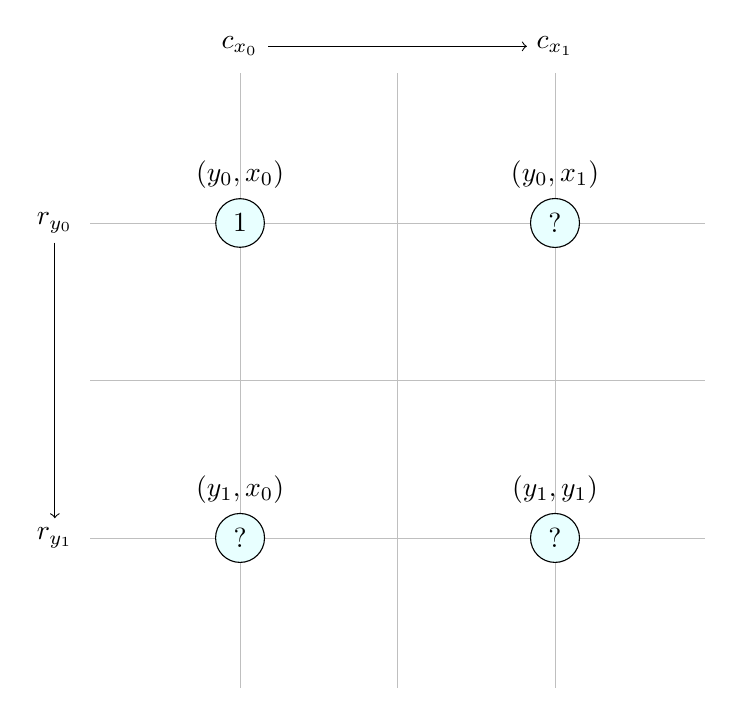
\begin{tikzpicture}[decoration={
    markings,
    mark=at position 1 with {\arrow[scale=1]{angle 90}};
  }]
  \draw[opacity=.5,help lines,step=2] (0.1,0.1) grid (7.9,7.9);
  \node[circle,draw,fill=bubbles,minimum size=0.5cm,label=above:{$(y_0,x_0)$}] at (2,6) {$1$};
    \node[circle,draw,fill=bubbles,minimum size=0.5cm,label=above:{$(y_0,x_1)$}] at (6,6) {?};
    \node[circle,draw,fill=bubbles,minimum size=0.5cm,label=above:{$(y_1,x_0)$}] at (2,2) {?};
    \node[circle,draw,fill=bubbles,minimum size=0.5cm,label=above:{$(y_1,y_1)$}] at (6,2) {?};
    \node[left] (r1) at (0,6) {${r_{y_0}}$};
    \node[left] (r2) at (0,2) {${r_{y_1}}$};
    \node[above] (c1) at (2,8) {${c_{x_0}}$};
    \node[above] (c2) at (6,8) {${c_{x_1}}$};
    \draw[->] (r1) -- (r2);
    \draw[->] (c1) -- (c2);
\end{tikzpicture}

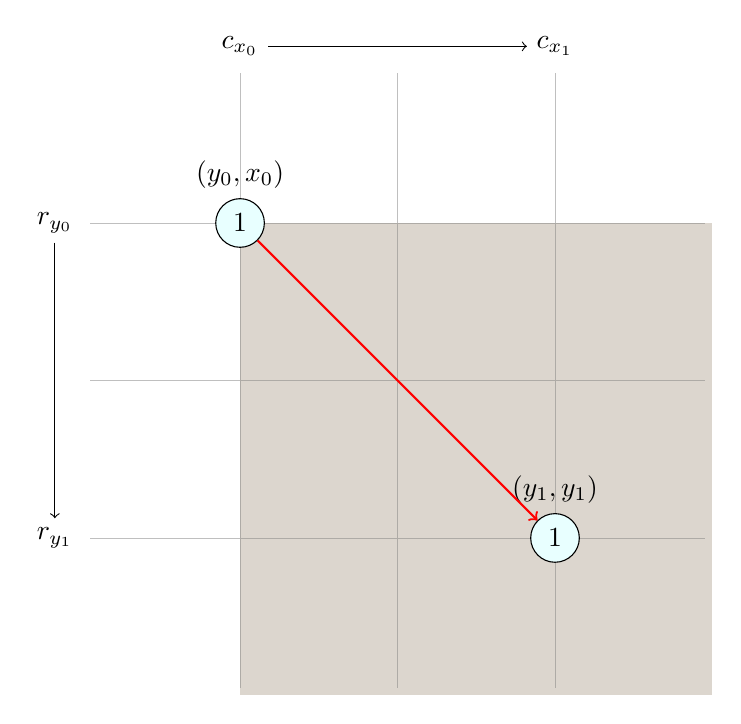
\begin{tikzpicture}[decoration={
    markings,
    mark=at position 1 with {\arrow[scale=1]{angle 90}};
  }]
  \fill[opacity=.3,color=shadow] (2,6) rectangle (8,0);
  \draw[opacity=.5,help lines,step=2] (0.1,0.1) grid (7.9,7.9);
  \node[circle,draw,fill=bubbles,minimum size=0.5cm,label=above:{$(y_0,x_0)$}] (start) at (2,6) {$1$};
  \node[circle,draw,fill=bubbles,minimum size=0.5cm,label=above:{$(y_1,y_1)$}] (end) at (6,2) {$ 1$};
    \node[left] (r1) at (0,6) {${r_{y_0}}$};
    \node[left] (r2) at (0,2) {${r_{y_1}}$};
    \node[above] (c1) at (2,8) {${c_{x_0}}$};
    \node[above] (c2) at (6,8) {${c_{x_1}}$};
    \draw[->] (r1) -- (r2);
    \draw[->] (c1) -- (c2);
    \draw[->,red,thick] (start) -- (end);
\end{tikzpicture}

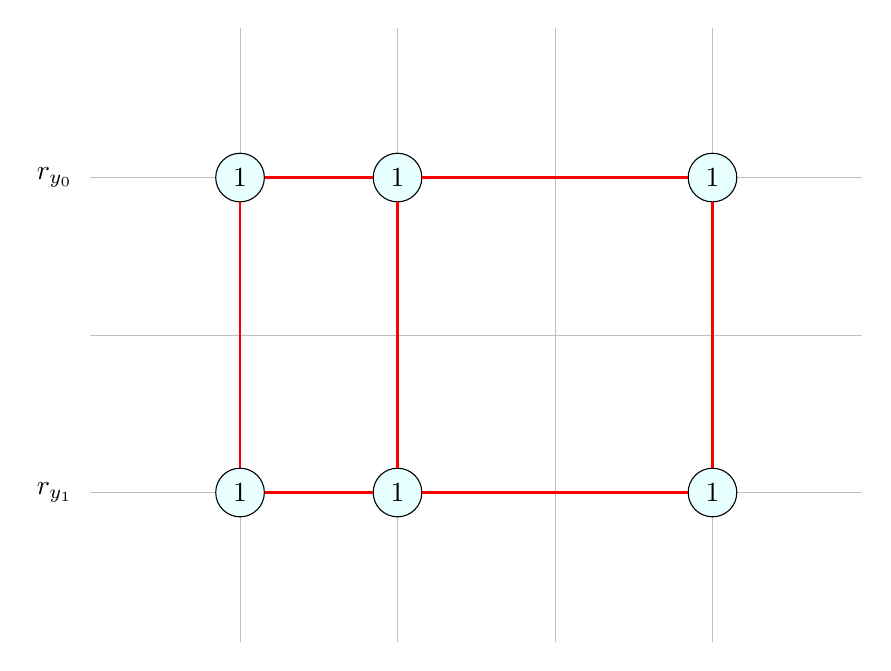
\begin{tikzpicture}[decoration={
    markings,
    mark=at position 1 with {\arrow[scale=1]{angle 90}};
  }]
  \draw[opacity=.5,help lines,step=2] (0.1,0.1) grid (9.9,7.9);
  \node[circle,draw,fill=bubbles,minimum size=0.5cm] (x1) at (2,6) {$1$};
  \node[circle,draw,fill=bubbles,minimum size=0.5cm] (x2) at (4,6) {$1$};
  \node[circle,draw,fill=bubbles,minimum size=0.5cm] (x3) at (8,6) {$1$};
  \node[circle,draw,fill=bubbles,minimum size=0.5cm] (y1) at (2,2) {$1$};
  \node[circle,draw,fill=bubbles,minimum size=0.5cm] (y2) at (4,2) {$1$};
  \node[circle,draw,fill=bubbles,minimum size=0.5cm] (y3) at (8,2) {$1$};
    \node[left] (r1) at (0,6) {${r_{y_0}}$};
    \node[left] (r2) at (0,2) {${r_{y_1}}$};
    \draw[red,thick] (x1) -- (y1);
    \draw[red,thick] (x2) -- (y2);
    \draw[red,thick] (x3) -- (y3);
    \draw[red,thick] (x1) -- (x2);
    \draw[red,thick] (x2) -- (x3);
    \draw[red,thick] (y1) -- (y2);
    \draw[red,thick] (y2) -- (y3);
\end{tikzpicture}


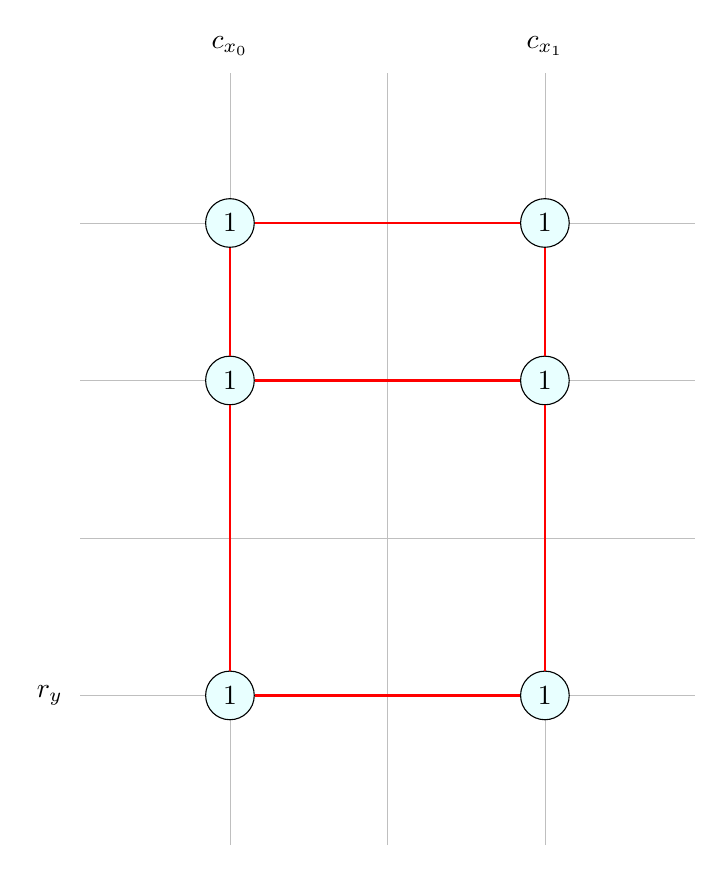
\begin{tikzpicture}[decoration={
    markings,
    mark=at position 1 with {\arrow[scale=1]{angle 90}};
  }]
\draw[opacity=.5,help lines,step=2] (0.1,0.1) grid (7.9,9.9);
  \node[circle,draw,fill=bubbles,minimum size=0.5cm] (x1) at (2,8) {$1$};
  \node[circle,draw,fill=bubbles,minimum size=0.5cm] (x2) at (2,6) {$1$};
  \node[circle,draw,fill=bubbles,minimum size=0.5cm] (x3) at (2,2) {$1$};
  \node[circle,draw,fill=bubbles,minimum size=0.5cm] (y1) at (6,8) {$1$};
  \node[circle,draw,fill=bubbles,minimum size=0.5cm] (y2) at (6,6) {$1$};
  \node[circle,draw,fill=bubbles,minimum size=0.5cm] (y3) at (6,2) {$1$};
  \node[left] (r1) at (0,2) {${r_y}$};
  \node[above] (c1) at (2,10) {${c_{x_0}}$};
  \node[above] (c2) at (6,10) {${c_{x_1}}$};
  \draw[red,thick] (x1) -- (y1);
  \draw[red,thick] (x2) -- (y2);
  \draw[red,thick] (x3) -- (y3);
  \draw[red,thick] (x1) -- (x2);
  \draw[red,thick] (x2) -- (x3);
  \draw[red,thick] (y1) -- (y2);
  \draw[red,thick] (y2) -- (y3);
\end{tikzpicture}

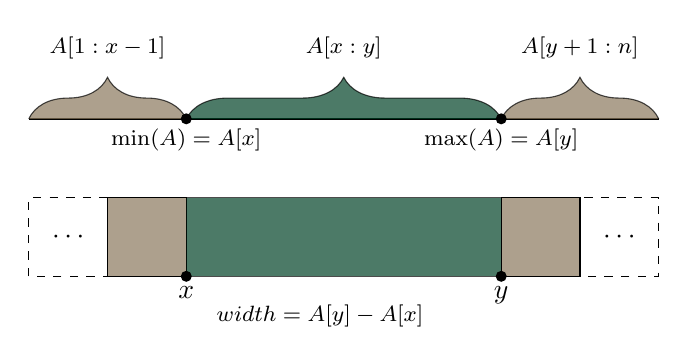
\begin{tikzpicture}[decoration={
    markings,
    mark=at position 1 with {\arrow[scale=1]{angle 90}};
  }]
\draw[thick] (0,0) -- (8,0);
% \draw (2,.5) -- (2,-.5) node[below] {$x$};
% \draw (6,.5) -- (6,-.5) node[below] {$y$};

\filldraw [decorate,decoration={brace,amplitude=15pt},fill=britishracinggreen,opacity=.7]
(2,0) -- (6,0) node [black,midway,yshift=.9cm,opacity=1] {\footnotesize $A[x:y]$};

\filldraw [decorate,decoration={brace,amplitude=15pt},fill=shadow,opacity=.7]
(0,0) -- (2,0) node [black,midway,yshift=.9cm,opacity=1] {\footnotesize $A[1:x-1]$};

\filldraw [decorate,decoration={brace,amplitude=15pt},fill=shadow,opacity=.7]
(6,0) -- (8,0) node [black,midway,yshift=.9cm,opacity=1] {\footnotesize $A[y+1:n]$};

\fill[black] (2,0)  circle (.07) node[below] {\footnotesize $\min(A)=A[x]$};
\fill[black] (6,0)  circle (.07) node[below] {\footnotesize $\max(A)=A[y]$};

\draw[dashed] (0,-2) rectangle node {$\cdots$} (1,-1);
\filldraw[fill=shadow,fill opacity=.7] (1,-2) rectangle (2,-1);
\filldraw[fill=britishracinggreen,opacity=.7] (2,-2) rectangle (6,-1);
\filldraw[fill=shadow,fill opacity=.7] (6,-2) rectangle (7,-1);
\draw[dashed] (7,-2) rectangle node {$\cdots$} (8,-1);
\fill[black] (2,-2)  circle (.07) node[below] {$x$};
\fill[black] (6,-2)  circle (.07) node[below] {$y$};
\node at (3.7,-2.5) {\footnotesize $width=A[y]-A[x]$};
\end{tikzpicture}

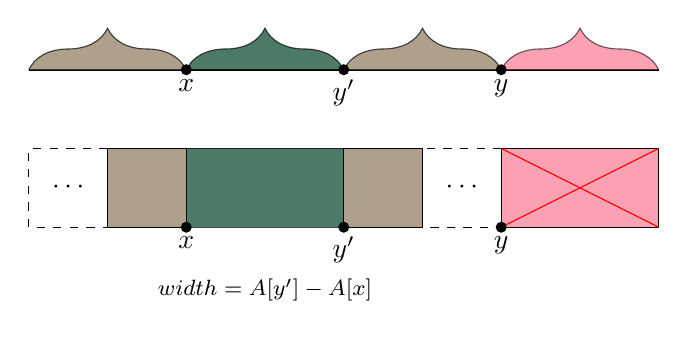
\begin{tikzpicture}[decoration={
    markings,
    mark=at position 1 with {\arrow[scale=1]{angle 90}};
  }]
\draw[thick] (0,0) -- (8,0);

\filldraw [decorate,decoration={brace,amplitude=15pt},fill=britishracinggreen,opacity=.7]
(2,0) -- (4,0);

\filldraw [decorate,decoration={brace,amplitude=15pt},fill=shadow,opacity=.7]
(0,0) -- (2,0);

\filldraw [decorate,decoration={brace,amplitude=15pt},fill=shadow,opacity=.7]
(4,0) -- (6,0);

\filldraw [decorate,decoration={brace,amplitude=15pt},fill=brinkpink,opacity=.6]
(6,0) -- (8,0);

\fill[black] (2,0)  circle (.07) node[below] {$x$};
\fill[black] (4,0)  circle (.07) node[below] {$y'$};
\fill[black] (6,0)  circle (.07) node[below] {$y$};

\draw[dashed] (0,-2) rectangle node {$\cdots$} (1,-1);
\filldraw[fill=shadow,fill opacity=.7] (1,-2) rectangle (2,-1);
\filldraw[fill=britishracinggreen,opacity=.7] (2,-2) rectangle (4,-1);
\filldraw[fill=shadow,fill opacity=.7] (4,-2) rectangle (5,-1);
\draw[dashed] (5,-2) rectangle node {$\cdots$} (6,-1);
\filldraw[fill=brinkpink,fill opacity=.6] (6,-2) rectangle (8,-1);
\draw[red] (6,-2) -- (8,-1);
\draw[red] (6,-1) -- (8,-2);
\fill[black] (2,-2)  circle (.07) node[below] {$x$};
\fill[black] (4,-2)  circle (.07) node[below] {$y'$};
\fill[black] (6,-2)  circle (.07) node[below] {$y$};
\node at (3,-2.8) {\footnotesize $width=A[y']-A[x]$};
\end{tikzpicture}

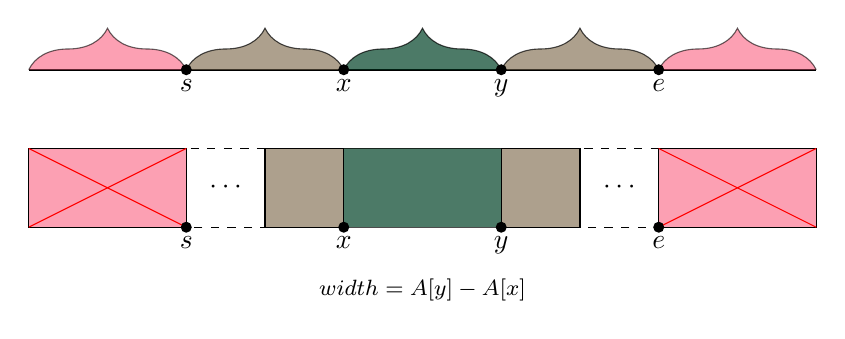
\begin{tikzpicture}[decoration={
    markings,
    mark=at position 1 with {\arrow[scale=1]{angle 90}};
  }]
\draw[thick] (-2,0) -- (8,0);

\filldraw [decorate,decoration={brace,amplitude=15pt},fill=britishracinggreen,opacity=.7]
(2,0) -- (4,0);

\filldraw [decorate,decoration={brace,amplitude=15pt},fill=shadow,opacity=.7]
(0,0) -- (2,0);

\filldraw [decorate,decoration={brace,amplitude=15pt},fill=shadow,opacity=.7]
(4,0) -- (6,0);

\filldraw [decorate,decoration={brace,amplitude=15pt},fill=brinkpink,opacity=.6]
(6,0) -- (8,0);

\filldraw [decorate,decoration={brace,amplitude=15pt},fill=brinkpink,opacity=.6]
(-2,0) -- (0,0);

\fill[black] (0,0)  circle (.07) node[below] {$s$};
\fill[black] (2,0)  circle (.07) node[below] {$x$};
\fill[black] (4,0)  circle (.07) node[below] {$y$};
\fill[black] (6,0)  circle (.07) node[below] {$e$};

\filldraw[fill=brinkpink,fill opacity=.6] (-2,-2) rectangle (0,-1);
\draw[dashed] (0,-2) rectangle node {$\cdots$} (1,-1);
\filldraw[fill=shadow,fill opacity=.7] (1,-2) rectangle (2,-1);
\filldraw[fill=britishracinggreen,opacity=.7] (2,-2) rectangle (4,-1);
\filldraw[fill=shadow,fill opacity=.7] (4,-2) rectangle (5,-1);
\draw[dashed] (5,-2) rectangle node {$\cdots$} (6,-1);
\filldraw[fill=brinkpink,fill opacity=.6] (6,-2) rectangle (8,-1);
\draw[red] (6,-2) -- (8,-1);
\draw[red] (6,-1) -- (8,-2);
\draw[red] (-2,-2) -- (0,-1);
\draw[red] (-2,-1) -- (0,-2);
\fill[black] (0,-2)  circle (.07) node[below] {$s$};
\fill[black] (2,-2)  circle (.07) node[below] {$x$};
\fill[black] (4,-2)  circle (.07) node[below] {$y$};
\fill[black] (6,-2)  circle (.07) node[below] {$e$};
\node at (3,-2.8) {\footnotesize $width=A[y]-A[x]$};
\end{tikzpicture}

\end{document}
